\chapter{Βιβλιογραφική Αναζήτηση Τεχνολογιών Αιχμής}
\label{chapter:state_of_the_art}

Πριν αναλυθεί η υλοποίηση του συστήματος που δημιουργήσαμε για την Ενεργή Παρακολούθηση
Eφαρμογών ως Υπηρεσίες (SaaS) και ιστοσελιδών που εδρεύουν στο διαδίκτυο, θα πασουσιάσουμε τεχνολογίες
που έχουν χτιστεί ήδη για το σκοπό αυτό και θα δείξουμε τους τομείς στους οποίους
διαφέρει το δικό μας σύστημα.

Εφαρμογές τέτοιου τύπου έχουν αναπτυχθεί κυρίως από εταιρίες αλλά υπάρχουν πολλά open source
project μικρότερου βεληνεκούς που επιτυγχάνουν τον ίδιο στόχο. Στη συνέχεια θα αναφερθούμε κυρίως στα
πιο γνωστά και διαδεδομένα εργαλεία παρουσιάζοντας τα δυνατά τους σημεία και περιγράφοντας τις λειτουργίες
που παρέχουν.

\begin{itemize}
	\item \textbf{Better Uptime}: Προσφέρει εύκολη ενσωμάτωση των ιστοσελιδών που θέλει κανείς να παρακολουθήσει.
	      Λειτουργεί κάνοντας ping κάθε τριάντα δευτερόλεπτα στο url που ορίζει ο χρήστης και παρουσιάζει
	      τα παραγόμενα δεδομένα σε ευπαρουσίαστα διαγράμματα (\autoref{fig:better_uptime}). Ένα από τα μεγάλα πλεονεκτήματα που έχει αφορά
	      τη δυνατότητα για πολλαπλά ping από διαφορετικές περιοχές του κόσμου (Ευρώπη, Ασία, Βόρεια Αμερική, Αυστραλία)
	      ώστε οι χρήστες να διαθέτουν μία πιο πλήρη εποπτεία του υπό μελέτη συστήματος/ιστοσελίδας. Αξίζει να σημειωθεί
	      ότι παρέχει και μηχανισμούς ενημέρωσης για να ειδοποιεί το χρήστη σε περίπτωση μη απόκρισης τους συστήματος, μέσα
	      από mail, εφαρμογές chatting και τηλεφωνικών κλήσεων.
	      \begin{figure}[!ht]
		      \centering
		      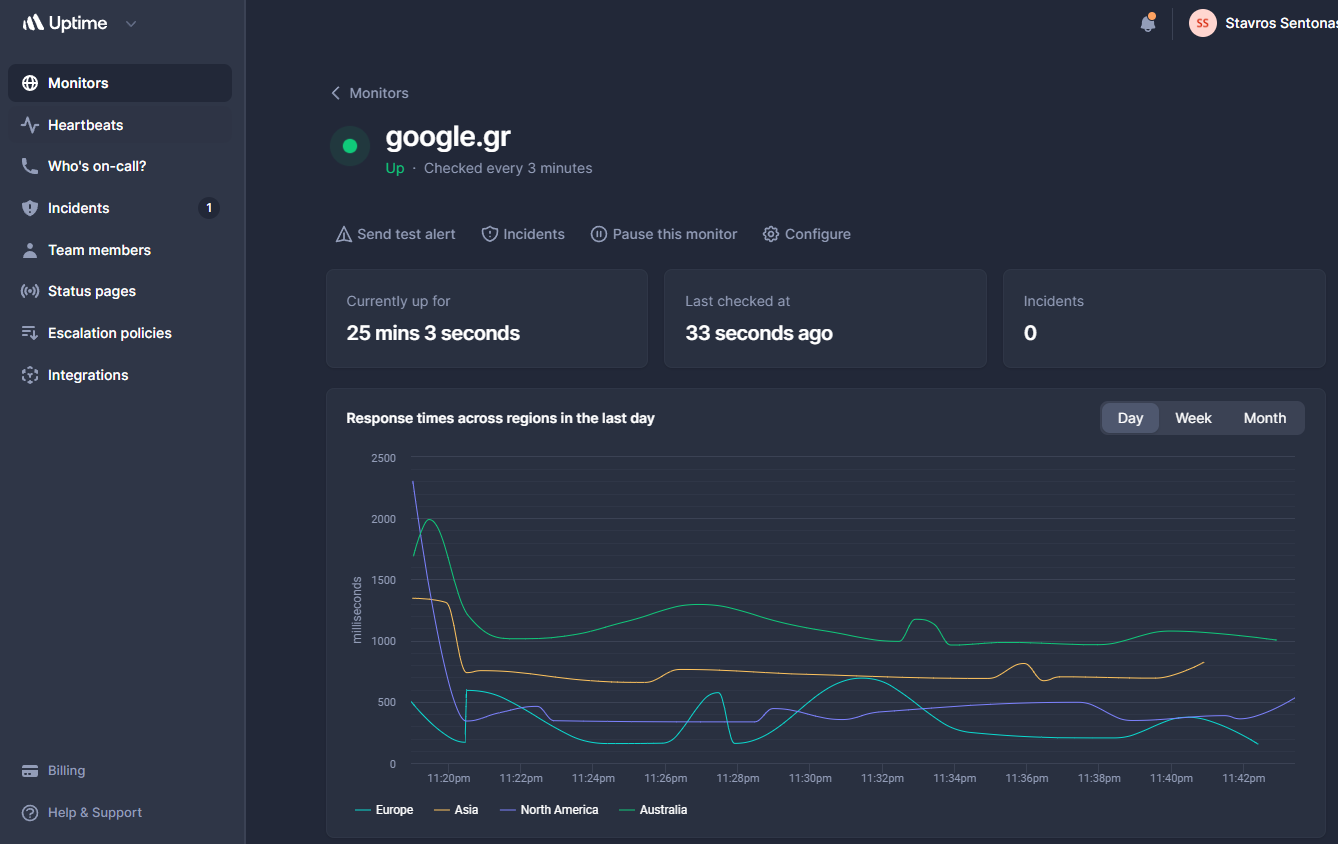
\includegraphics[width=0.7\textwidth]{./images/chapter3/better-uptime.png}
		      \caption[Παράδειγμα χρήσης του εργαλείου Better Uptime]{Παράδειγμα χρήσης του εργαλείου Better Uptime}
		      \label{fig:better_uptime}
	      \end{figure}
	\item \textbf{Uptime Robot}: Επιτρέπει πέρα από την επιλογή του url και την επιλογή παραπάνων παραμέτρων που επηρεάζουν
	      την απάντηση που θα επιστρέψει το υπό μελέτη σύστημα. Οι παράμετροι αυτοί σχετίζονται με τους headers του μηνύματος που
	      αποστέλλεται και πιο συγκεκριμένα με αυτούς που αφορούν την αυθεντικοποίηση του χρήστη (στην προκειμένου περίπτωση
	      του συστήματος παρακολούθησης). Πέρα από αυτά μπορεί να καθορίσει την επιθυμητή http κατάσταση της απόκρισης
	      της ιστόσελίδας και το χρόνο που θα παρεμβάλλεται μεταξύ διαδοχικών αιτημάτων (pings). Τέλος διαθέτει κάποια βασικά διαγράμματα
	      που σχετίζονται με το αν η απόκριση του συστήματος είναι ορθή ή όχι (\autoref{fig:uptime_robot})
	      \begin{figure}[!ht]
		      \centering
		      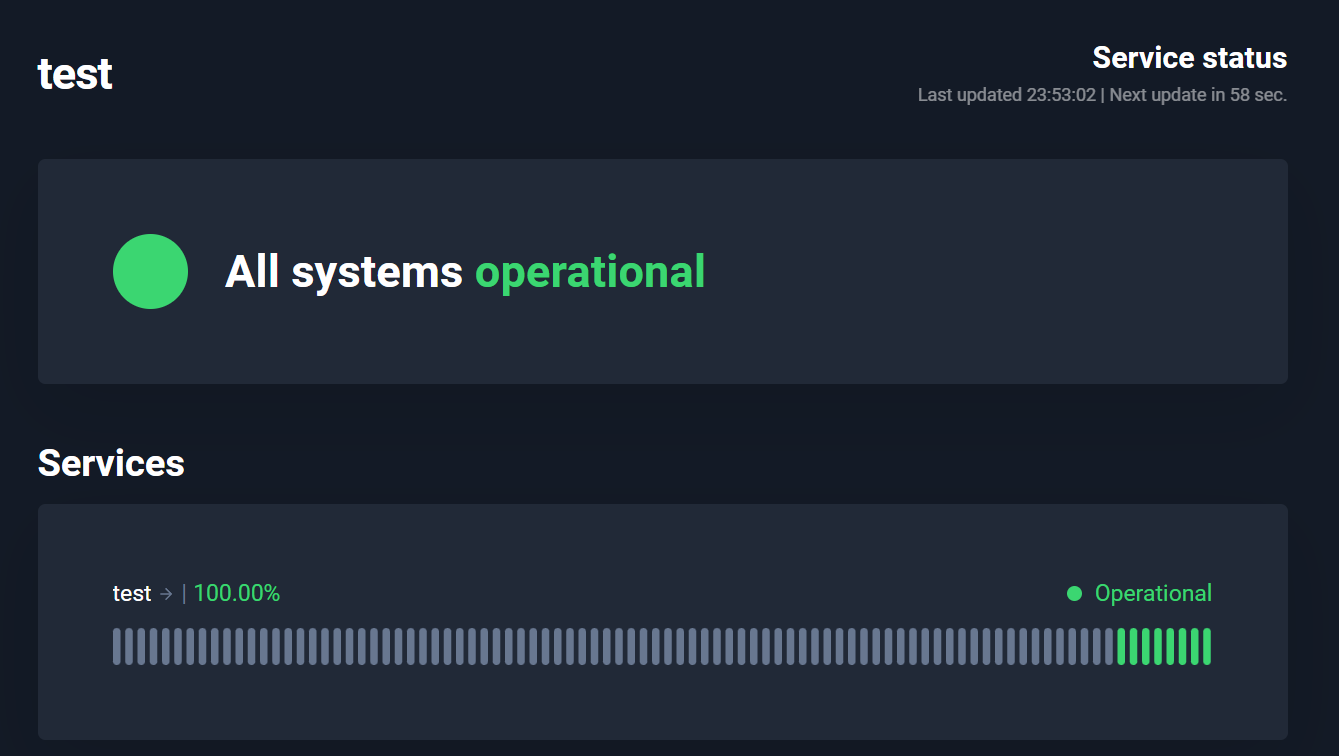
\includegraphics[width=0.7\textwidth]{./images/chapter3/uptime_robot.png}
		      \caption[Παράδειγμα χρήσης του εργαλείου Uptime Robot]{Παράδειγμα χρήσης του εργαλείου Uptime Robot}
		      \label{fig:uptime_robot}
	      \end{figure}
	\item \textbf{Site24x7}: Διαθέτει μετρικές, που αφορούν τη μέγιστη, ελάχιστη τιμή του χρόνου απόκρισης του συστήματος, καθώς και τη μέση τιμή του,
	      ενώ παράλληλα δίνει μία εικόνα του throughput του συστήματος. Δεν λείπει φυσικά και ένα διάγραμμα απόκρισης χρόνου (\autoref{fig:site24x7})
	      που καθιστα τα δεδομένα που συλλέγονται πιο εύκολα στην κατανόηση και οπτικοποίηση.
	      \begin{figure}[!ht]
		      \centering
		      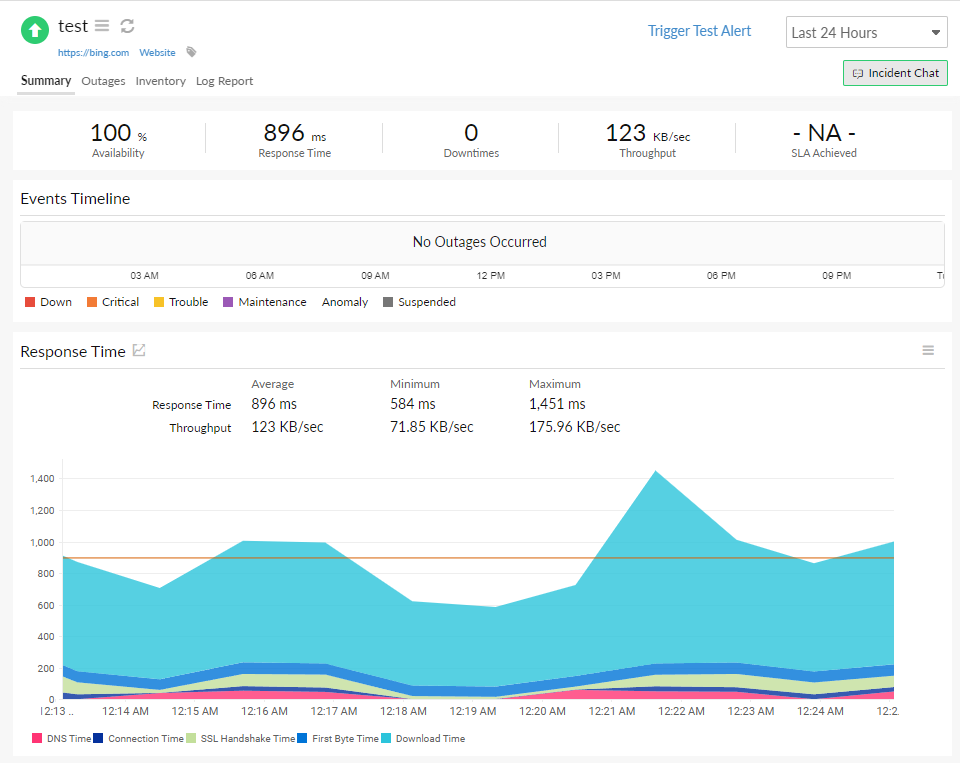
\includegraphics[width=0.7\textwidth]{./images/chapter3/site24x7.png}
		      \caption[Παράδειγμα χρήσης του εργαλείου Site24x7]{Παράδειγμα χρήσης του εργαλείου Site24x7}
		      \label{fig:site24x7}
	      \end{figure}
	\item \textbf{Uptimia}: Πέρα από τα κλασικού τύπου http αιτήματα μπορεί να κάνει ελέγχους παρακολούθησης (uptime monitoring)
	      σε DNS, UDP, TCP και email με απόσταση έως και τριάντα δευτερολέπτων (μεταξύ αιτημάτων). Αξίζει να σημειωθεί ότι η συγκεκριμένη
	      εφαρμογή έχει δυνατότες και παθητικής παρακολούθησης (RUM). Αρχικά επιλέγουμε το site το οποίο θέλουμε να παρακολουθήσουμε
	      καθώς και τα δεδομένα για τα οποία θέλουμε να ενημερωνόμαστε/παρακολουθούμε. Αυτά σχετίζονται κυρίως με σφάλματα ή
	      καταστάσεις στις οποίες βρίσκεται το σύστημα και μπορεί να δηλώνουν κάποιο πρόβλημα. Καταστάσεις όπως η μειωμένη απόδοση του συστήματος
	      εξαιτίας του χρόνου που παίρνει για να φορτώσει δεδομένα ή η απότομη πτώση του πλήθους των χρηστών μίας σελίδας.
	      Για να επιτύχει τέτοιας μορφής ελέγχους παράγει (ανάλογα με τον τύπο των ελέγχων που επιλέγουμε)
	      ένα script γραμμένο σε JavaScript που τοποθείται στην αρχή της ιστοσελίδας την οποία θέλουμε να παρακολουθήσουμε.
	      Με αυτό τον τρόπο έχουν τη δυνατότητα συλλογής δεδομένων πραγματικών χρηστών.
	      \begin{figure}[!ht]
		      \centering
		      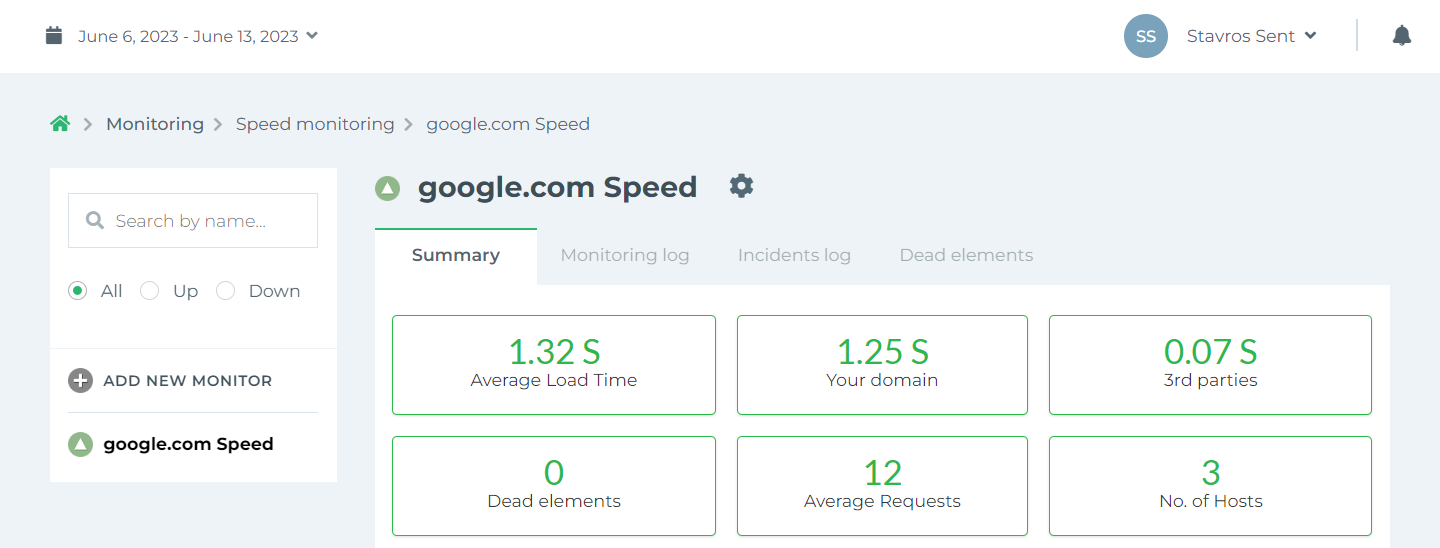
\includegraphics[width=0.7\textwidth]{./images/chapter3/uptimia.png}
		      \caption[Παράδειγμα χρήσης του εργαλείου Uptimia]{Παράδειγμα χρήσης του εργαλείου Uptimia}
		      \label{fig:uptimia}
	      \end{figure}
\end{itemize}

\break

Παραπάνω αναφέρθηκαν μερικά μόνο κάποια από τα εργαλεία που υπάρχουν σήμερα για την Ενεργη Παρακολούθηση του Χρόνου
και Απόκρισης Ιστοτόπων και Διαδικτυακών Εφαρμογών. Σε αυτά θα πρέπει να προστεθούν πληθώρα εφαρμογών όπως τα:
\textbf{StatusCake}, \textbf{SemaText}, \textbf{Uptrends}, \textbf{Dotcom-monitor}, \textbf{Updown}, \textbf{Datadog Synthetics}.
Οι δυνατότες που προσφέρουν ως επί το πλείστον μπορούν περιγραφούν πλήρως από όσα αναπτύξαμε προηγουμένως, για αυτό το λόγω δεν θα αναφερθούμε περαιτέρω.

Πρέπει σε αυτό το σημείο όμως να τονίσουμε ότι όσα προαναφέρθηκαν αποτελούν προϊόντα εταιριών.
Αυτό όμως δεν σταματάει την ανάπτυξη open source projects που υλοποιήθηκαν από χρήστες είτε ως προσωπικά project, είτε
ως project μίας μεγαλύτερης ομάδας από developers. Έτσι και στο πλαίσιο της Ενεργής Παρακολούθησης μερικά από τα πιο
γνωστά και δημοφιλή μεταξύ developers αποθετήρια αποτελούν τα:

\begin{itemize}
	\item \href{https://github.com/upptime/upptime}{Upptime}: Αποτελεί μία ενδιαφέρουσα προσέγγιση στο πρόβλημα
	      της διαχείρησης των schedulers που θα πρέπει να έχει το σύστημα για να κάνει αιτήματα ανά ένα συγκεκριμένο
	      και σταθερό χρονικό διάστημα. Προκειμένου να επιτύχει κάτι τέτοιο αξιοποιεί τις δυνατότητες του GitHub (cloud-based υπηρεσία αποθήκευσης git αποθετηρίων)
	      και των actions που αυτό σου επιτρέπει να εκτελείς κάθε πέντε λεπτά. Έτσι λοιπόν ανά πέντε λεπτά (ελάχιστος χρόνος ελέγχου απόκρισης)
	      τρέχει αυτοματοποιημένα και μέσω του GitHub (ανεξάρτητα από το σύστημα αυτό) μία διαδικασία που κάνει αιτήματα στην σελίδα που ο χρήστης ορίζει.
	      Φυσικά τα αποτελέσματα αυτά αποθηκεύονται και ανά έξι ώρες παράγονται διαγράμματα που μπορείς να τα δεις μέσα από μία σελίδα που παράγεται αυτόματα.
	      \begin{figure}[!ht]
		      \centering
		      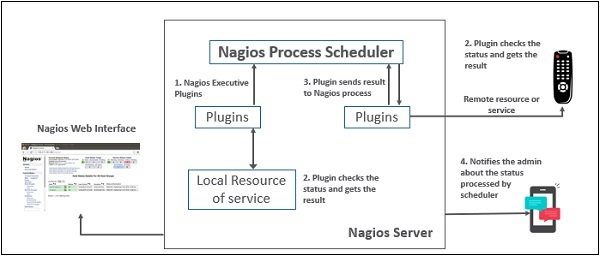
\includegraphics[width=0.8\textwidth]{./images/chapter3/nagios.jpg}
		      \caption[Αρχιτεκτόνική Συστήματος Nagios]{Αρχιτεκτόνική Συστήματος Nagios}
		      \label{fig:nagios}
	      \end{figure}
	\item \href{https://github.com/NagiosEnterprises/nagioscore}{Nagios}: Είναι ένα πρόγραμμα γραμμένο στη γλώσσα προγραμματισμού
	      C. Πέρα από το backend, που θα δούμε στη συνέχεια διαθέτει και Γραφικό Περιβάλλον Χρήστη (Graphical User Interface - GUI).
	      Αποτελείται από ένα σύστημα ενός server (nagios server), oποίος λειτουργεί σαν ένας scheduler που στέλνει σήματα
	      για να ξεκινήσει την εκτέλεση plugins στα απομακρυσμένα συστήματα που θέλουμε να παρακολουθήσουμε. Μόλις τα plugins δεχτούν
	      απάντηση επιστρέφουν στον server o οποίος προωθεί την πληροφορία στο GUI για να τη δούνε και οι χρήστες. Δεν χρησιμοποιείται κάποια βάση
	      δεδομένων, καθώς η πληροφορία που μαζεύεται αποθηκεύεται μόνο σε logs στο σύστημα που τρέχει την υπηρεσία αυτή. Την αρχιτεκτονική σου συστήματος μπορούμε
		  δούμε στην \autoref{fig:nagios}
	\item \href{https://github.com/louislam/uptime-kuma}{Kuma Uptime}: Αποτελεί μία εύκολή να χρησιμοποιήσεις και να στήσεις
	      self-hosted εφαρμογή γραμμένη σε JavaScript για Ενεργή Παρακολούθηση. Για την αποστολή των αιτημάτων σε απομακρυσμένες (στο διαδίκτυο) σελίδες
	      χρησιμοποιεί \textbf{child\_proccesses}, ένα api δήλαδή που περιλαμβάνει η Node.js για τη δημιουργία διεργασιών (processes) εντός άλλων διεργασιών.
	      Η εφαρμογή περιλαμβάνει backend και frontend, στο οποίο μπορείς να δεις τα αποτελέσματα του monitoring. Αξίζει να σημειωθεί
	      ότι τα δεδομένα αποθηκεύονται σε βάση SQLite, ένα προσωρινό σύνολο δεδομένων που υφίσταται μόνο στο πλαίσιο εκτέλεσης μίας εφαρμογής.
	      Αποτελεί μία server-less βάση δεδομένων και είναι άρρηκτα συνδεδεμένη με την εφαρμογή στην οποία υπάρχει.
	      \begin{figure}[!ht]
		      \centering
		      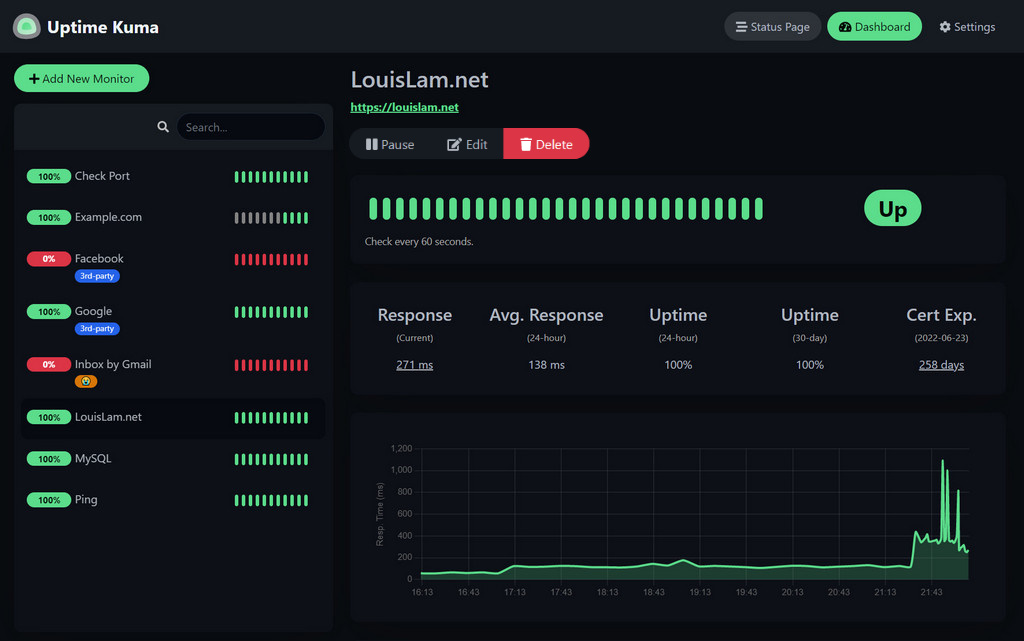
\includegraphics[width=0.7\textwidth]{./images/chapter3/kuma-uptime.jpg}
		      \caption[Παράδειγμα χρήσης του εργαλείου Kuma Uptime]{Παράδειγμα χρήσης του εργαλείου Kuma Uptime}
		      \label{fig:kuma_uptime}
	      \end{figure}
\end{itemize}

Κάθε σύστημα που αναφέρθηκε έχει πλεονεκτήματα αλλά και μειονεκτήματα σε σχέση με άλλα.
Αυτό που θέλαμε να διαθέτει ιδανικά ένα σύστημα Παρακολούθησης, βάση όλων αυτών που είδαμε μέχρι τώρα,
είναι τα εξής:

\begin{enumerate}
	\item Σταθερό και Αξιόπιστο σύστημα διαχείρησης προγραμματισμού (scheduling system) που θα
		καθορίζει το πότε πρέπει να ξεκινάνε τα αιτήματα προς τα εξωτερικά υπό παρακολούθηση συστήματα.
	\item Κάποια μορφή βάσης δεδομένων στην οποία θα αποθηκεύουμε τα δεδομένα που συλλέγουμε.
	\item Χρήση ιστορικών δεδομένων για τον υπολογισμό μετρικών στατιστικής φύσης σε βάθος χρόνου.
	\item Προβολή των δεδομένων σε ευπαρουσίαστα και εύπεπτα διαγράμματα που θα βοηθούν το χρήστη να αντιλαμβάνεται
		γρήγορα την κατάσταση των συστημάτων του
	\item Διάθεση τρόπων ειδοποίησης του χρήστη σε περίπτωση που κάποιο από τα συστήματα δεν ανταποκρίνεται
	\item Δυνατότητα για οριζόντια κλιμάκωση (\textbf{horizontal scaling})
	\item Ελαχιστοποίηση downtime του συστήματος 
	\item Πλήρης παραμετροποίηση του μηνύματος που αποστέλλεται (κατάλληλη ρύθμιση headers, body και query)
	\item Ρύθμιση του χρόνου μεταξύ διαδοχικών μυνημάτων
\end{enumerate}

Πολλές απο τις εφαρμογές που είδαμε καλύπτουν σε κάποιο βαθμό μερικά από τα παραπάνω, αλλά καμία
δεν τα καλύπτει όλα ταυτόχρονα. Τα εργαλεία που αναπτύχθηκαν στο πλαίσιο εταιριών έχουν δυνατότητες κλιμάκωσης
αλλά στα περισσότερα αν όχι σε όλα μπορείς να δεις πληροφορία μέχρι ένα συγκεκριμένο χρονικό διάστημα πίσω στο χρόνο,
κρύβοντας δεδομένα που είτε δεν αποθηκεύουν πλέον είτε δεν μπορούν να αντλήσουν αρκετά γρήγορα.
Απο την άλλη οι περισσότερες open source εφαρμογές που αναφέραμε δεν μπορούν να κάνουν τόσο εύκολα scaling
καθώς είναι φτιαγμένες να δουλεύουν για περιορισμένο πλήθος χρηστών. 

\begin{table}[H]
	\begin{center}
		\caption{Σύγκριση Εργαλείων Ενεργής Παρακολούθησης}
		\label{tab:active_monitoring_characteristics}
		\begin{tabular}{| p{40mm} | c | c | c | c | c | c |}
			\hline & \thead{Υλοποίηση \\ μας} & \thead{Better \\ Uptime} & \thead{Uptime \\ Robot} & \thead{Site24x7} & \thead{Uptimia} & \thead{Kuma} \tabularnewline
			\hline \thead{Σταθερότητα} & \checkmark & \checkmark & \checkmark & \checkmark & \checkmark & \checkmark \tabularnewline
			\hline \thead{Βάση Δεδομένων} & \checkmark  & \checkmark  & \checkmark & \checkmark & \checkmark & \tabularnewline
			\hline \thead{Ιστορικά Δεδομένα} & \checkmark & & & & & \tabularnewline
			\hline \thead{Διαγράμματα} & \checkmark & \checkmark & & \checkmark & \checkmark & \tabularnewline
			\hline \thead{Ειδοποιήσεις} & \checkmark & \checkmark & \checkmark & \checkmark & \checkmark & \checkmark \tabularnewline
			\hline \thead{Ελαχιστοποίηση \\ Downtime} & \checkmark & \checkmark & \checkmark & \checkmark & \checkmark & \checkmark \tabularnewline
			\hline \thead{Παραμετροποίηση \\ μηνυμάτων} & \checkmark & \checkmark & \checkmark & \checkmark & \checkmark & \tabularnewline
			\hline \thead{Ρύθμιση Χρόνου \\ μεταξύ μηνυμάτων} & \checkmark & \checkmark & \checkmark & \checkmark & \checkmark & \checkmark \tabularnewline
			\hline \thead{Οριζόντια \\ Κλιμάκωση} & \checkmark & \checkmark & \checkmark & \checkmark & \checkmark & \tabularnewline
			\hline
		\end{tabular}
	\end{center}
\end{table}

Στη διπλωματική αυτή εργασία λοιπόν καλούμαστε να δημιουργήσουμε ένα τέτοιο υπολογιστικό σύστημα
που θα καλύπτει τα προαναφερθέντα.
